\documentclass{ctexrep}
\bibliographystyle{plain}
\CTEXsetup[format={\Large\bfseries}]{section}
\usepackage{longtable}
\usepackage{graphicx}
\usepackage{url}
\usepackage{supertabular}
\usepackage{float}
\usepackage{multicol}
\usepackage[a4paper, inner=2.5cm, outer=4cm, top=2cm,bottom=3cm, bindingoffset=1cm]{geometry}
\usepackage{tabularx, makecell, multirow,ulem}
\usepackage{listings,xcolor}
\lstset{
	rulesepcolor= \color{gray}, %代码块边框颜色
	breaklines=true,  %代码过长则换行
	numbers=left, %行号在左侧显示
	numberstyle= \small,%行号字体
	keywordstyle= \color{red},%关键字颜色
	commentstyle=\color{gray}, %注释颜色
	frame=shadowbox%用方框框住代码块
}
\usepackage[bookmarks=true,colorlinks,breaklinks]{hyperref}
\title{\textbf{计算机网络自选实验报告} \\ [2ex] \begin{large} ns-3在多种网络环境下模拟vStomp协议 \end{large} }
\author{罗浩1752547,李一珉1752882\\江宵汉1752916,张子健1752894}
\date{}
\begin{document}
	\maketitle
	\tableofcontents
	
	\chapter{实验简介}
	\section{实验目的}
	本实验通过ns-3来模拟在实验室中难以搭建的网络基本结构(蜂窝LTE网络),并在应用层实现了vStomp\footnote{very Simple Text Oriented Messaging Protocol,将在后文进行详细描述}协议以支持类似于消息队列的聊天系统,并进行基本的可视化演示。通过本次实验,获得使用软件进行网络模拟的基本技能,并获得使用Socket实现一个简单应用层协议的体验。
	\section{实验设备与参考资料}
	\begin{itemize}
		\item ns-3.30.1软件包
		\item Stomp协议规范与参考实现 \url{http://stomp.github.io/}
		\item 《开源网络模拟器ns-3 - 架构与实践》
		\item 《ns-3网络模拟器基础及应用 》
	\end{itemize}
	\chapter{实验拓扑结构}
	
	\chapter{vStomp协议}
	\section{Stomp 协议简介}
	Stomp协议是一种简单而易于实现的协议,经常被用于\textbf{Websocket}协议上从而实现Web端的实时通信功能。在我们本学期的其他项目中,为了实现Web端的在线聊天功能,我们采用的就是Stomp协议,因此对于本协议所受到的广泛支持\footnote{前端可以直接使用JavaScript中相应的库而成为Stomp Client,后端Spring Boot框架中自带必要的支持,而类似于RabbitMQ、Kafka以及ActiveMQ这样的消息队列都提供了官方的插件成为高性能的 Stomp Server。}印象深刻,也正是这次接触使得我们决定在计算机网络实验的自选项目中尝试对本协议进行模拟。
	
	Stomp协议的全称是 \textbf{Simple Text Oriented Messaging Protocal},正如这个名字中所暗示的那样,它的设计哲学就是简明与可交互性,用户可以自主进行一系列约定从而达成自己的目标。因此每个部分的具体信息都相当灵活,使得Stomp可以被用于各种各样的系统之中。
	
	Stomp的帧格式如下:
	\begin{lstlisting}
COMMAND
header1:value1
header2:value2
header3:value3

bodyEOF
	\end{lstlisting}
	
	其中,COMMAND代表了这条消息的主要语义,而header中的键值对则补充了具体的语义,body是要传递的信息,EOF标志这帧的结束,例如SEND、SUBSCRIBE、UNSUBSCRIBE、CONNECT以及DISCONNECT。具体的列表可以参看Stomp的官网,这里就不再赘述。我们可以想象成用户在连接之后就可以收听不同的频道,也可以向各个频道发送信息,而收听该频道的所有用户都将会接受到相应的信息。在这里我们使用我们另一个项目\footnote{该项目是关于设计并实现一个社交网站,其中的一个重要功能就是在线聊天。}的例子在展示Stomp协议。在用户登录之后,我们将会自动为他建立 WebSocket连接,并完成与后端RabbitMQ的握手。具体的消息信息请查看截图 \ref{fig:stompdemo}。
	\begin{figure}[H]
		\centering
		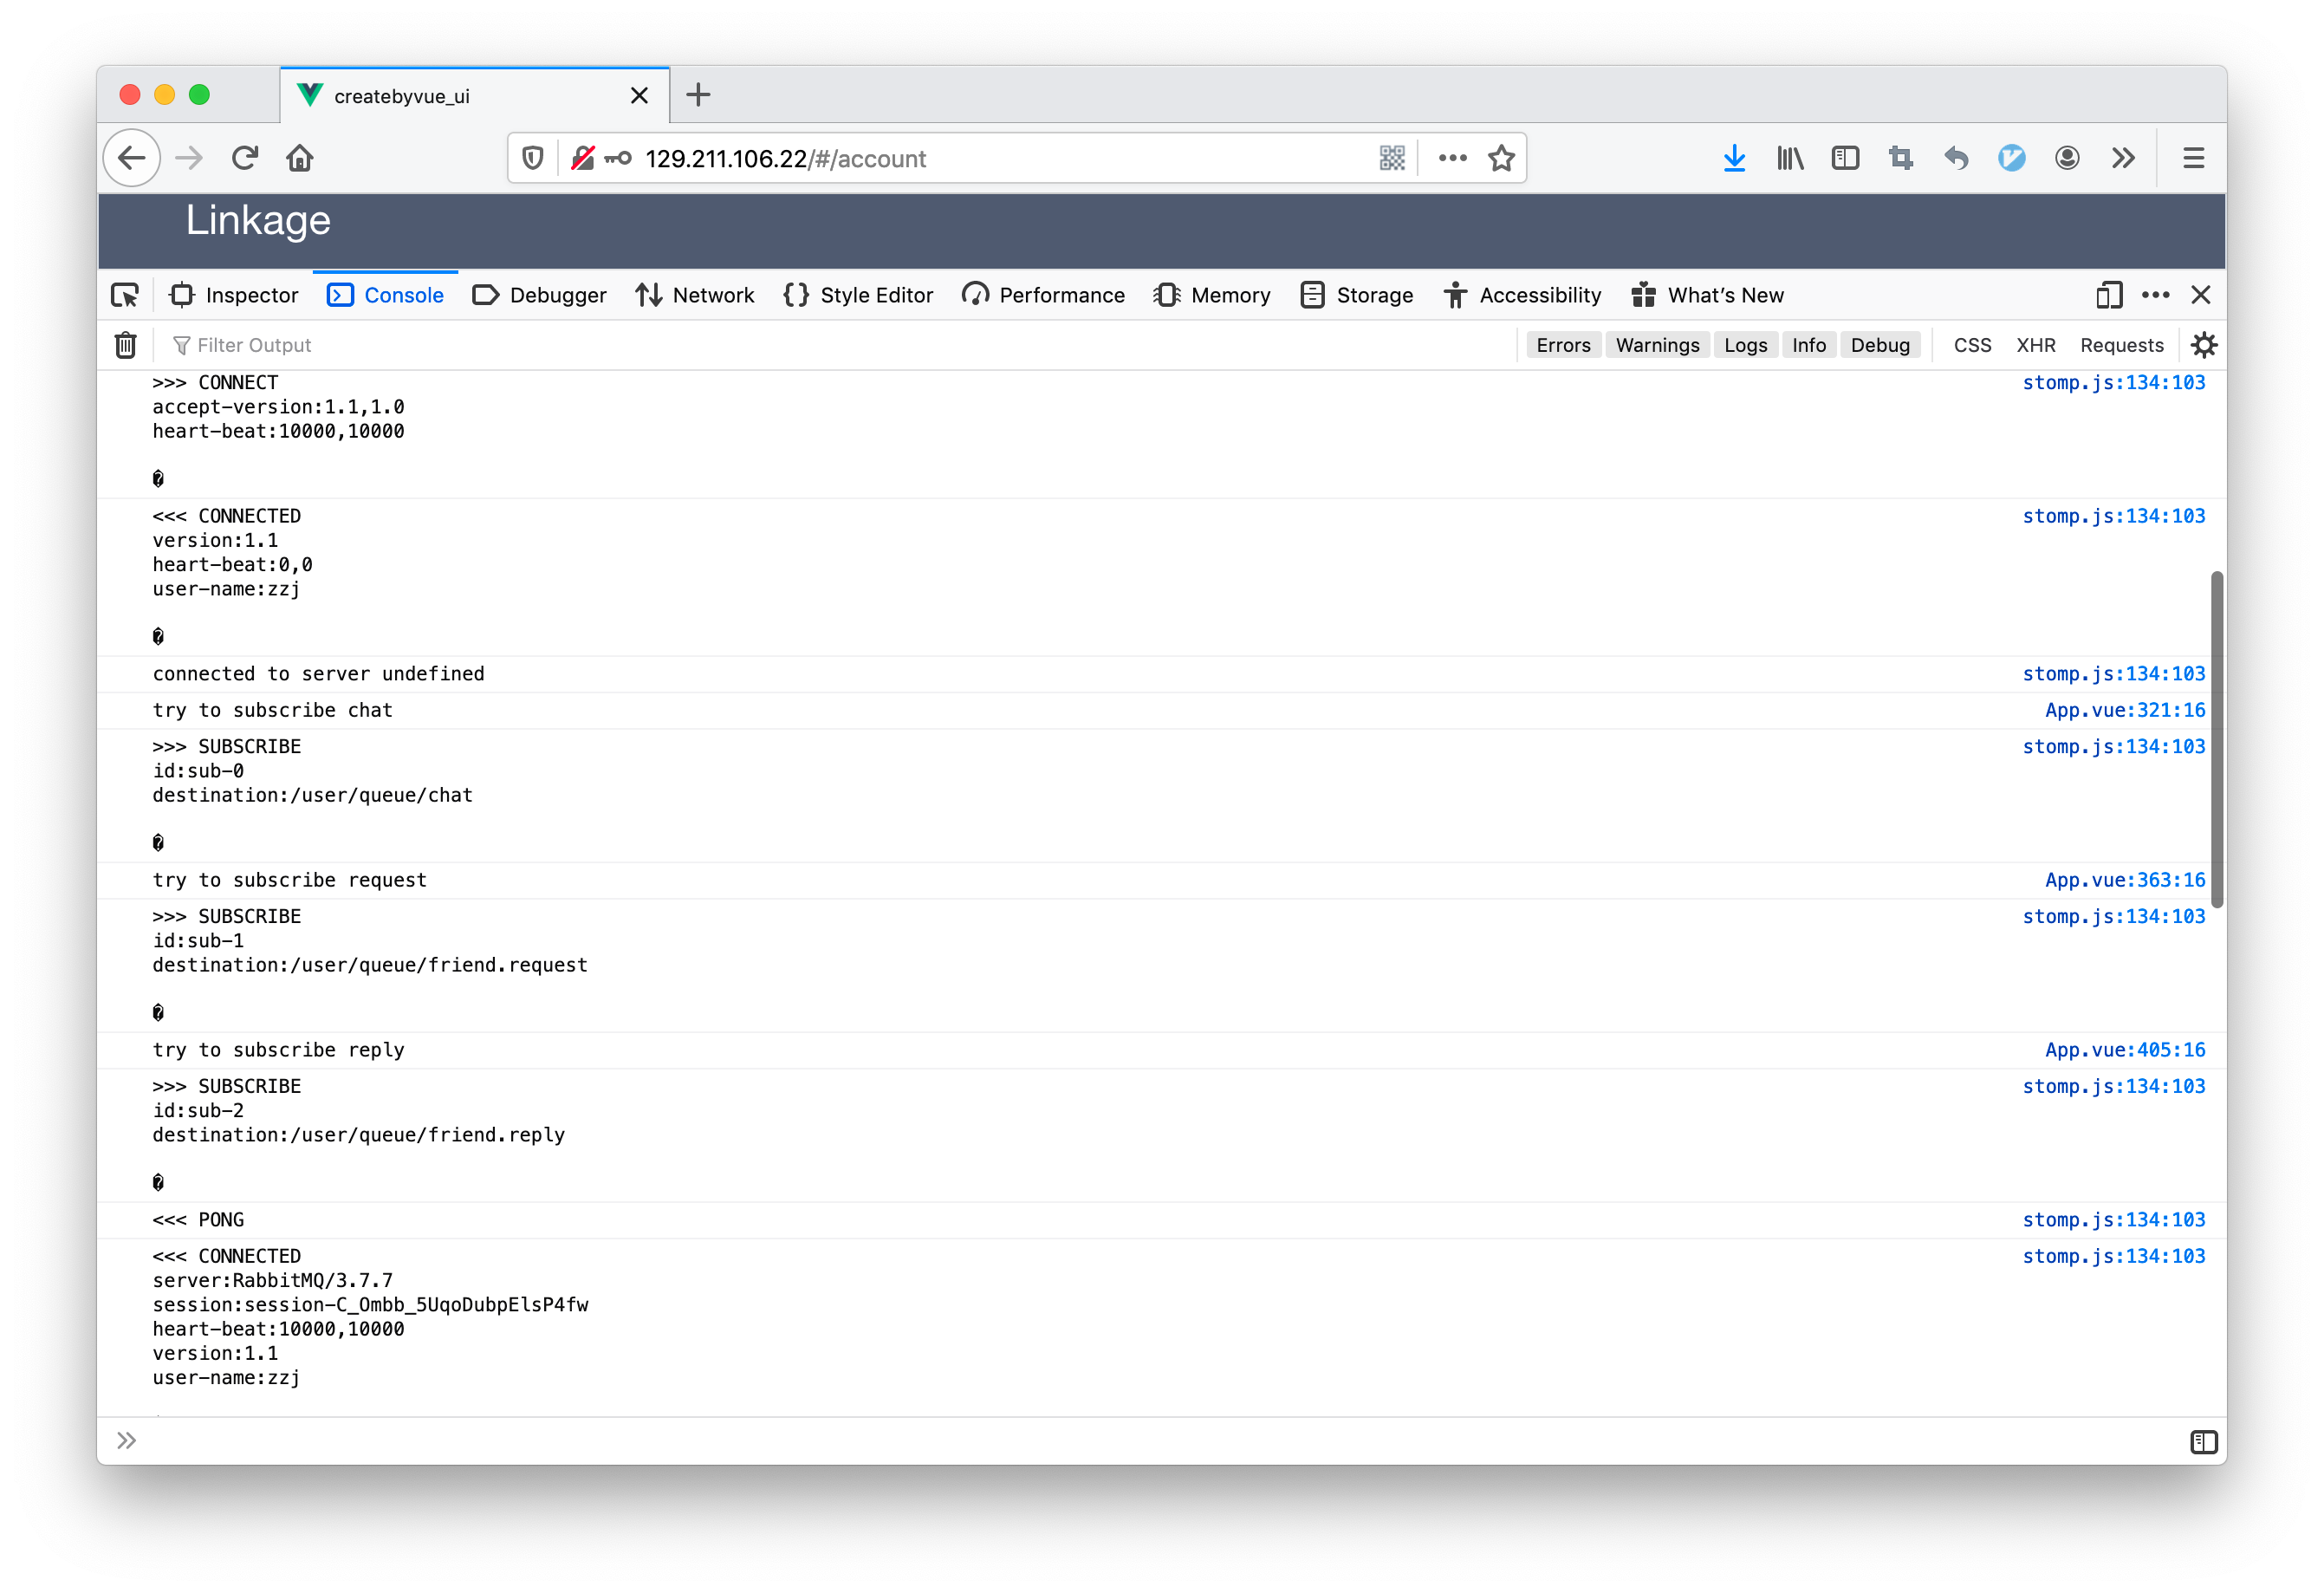
\includegraphics[width=0.9\linewidth]{img/stompDemo}
		\caption{Stomp 协议浏览器截图}
		\label{fig:stompdemo}
	\end{figure}
	\section{vStomp协议详述}
	在我们的自选实验中,我们对Stomp协议中一些不常用的功能进行了删除,对一些较为复杂对约定进行了简化之后,得到了我们自己的协议,我们生动的为之命名vStomp,very Simple Text Oriented Messaging Protocal。下面我们对各个命令做出说明
	\begin{enumerate}
		\item \textbf{CONNECT命令}。在用户初次进入系统时,需要向Server注册,发送以下格式的帧\begin{lstlisting}
CONNECT
name:x

		\end{lstlisting}该命令对应的语义为:\begin{enumerate}
			\item 名为x的用户向服务器注册。
			\item 服务器为该用户创建专门的频道,名字和用户名相同。
		\end{enumerate}
	\item \textbf{CONNECTED命令}。在服务器接受用户连接之后,向用户回复以下格式的帧\begin{lstlisting}
CONNECTED
	\end{lstlisting}该命令对应的语义为:\begin{enumerate}
		\item 服务器中已经保存了用户的信息。
		\item 用户可以进一步发送消息。
	\end{enumerate}
		\item  \textbf{DISCONNECT命令}。用户在完成会话之后,向服务器告知切断连接,发送以下格式的帧\begin{lstlisting}
DISCONNCT
name:x
		\end{lstlisting}该命令对应的语义为:\begin{enumerate}
			\item 名为x的用户将断开连接。
			\item 服务器将该用户从所有收听了的频道中移除。
		\end{enumerate}
		\item \textbf{SUBSCRIBE命令}。用户在完成连接之后,可以收听一些频道,发送以下格式的帧\begin{lstlisting}
SUBSCRIBE
channel:net
name:x
		\end{lstlisting}该命令对应的语义为:\begin{enumerate}
			\item 名为x的用户收听名为net的频道。
		\end{enumerate}
		\item \textbf{UNSUBSCRIBE 命令}。用户可以选择取消收听一些频道,发送以下格式的帧\begin{lstlisting}
UNSUBSCRIBE
channel:net
name:x
		\end{lstlisting}该命令对应的语义为:\begin{enumerate}
			\item 名为x的用户取消收听名为net的频道。
		\end{enumerate}
		\item \textbf{SEND 命令}。用户可以向频道发送一些信息,发送以下格式的帧\begin{lstlisting}
SEND
target:net

I love computer network. Challenging and interesting.
		\end{lstlisting}该命令的语义为:\begin{enumerate}
			\item 向net频道发送信息:“I love computer network. Challenging and interesting.”
			\item 所有收订本频道的用户都将收到本条信息。
		\end{enumerate}
	\end{enumerate}

可以看到,我们的vStomp协议可以支持基础的订阅者-发布者模式,我们的例子比较偏向于聊天,单人聊天在CONNECT命令之后就自动具备,而群聊可以通过共同收听某个频道来达成。虽然在我们的实现中信息都暂时是UTF-8的文本信息,但是拓展到二进制协议也是非常方便的。
	\chapter{vStomp实现}
	// 物理代码的描述
	
	下面叙述协议的整体工作方式。在物理层连接搭建完毕之后,我们会在其中一台机器上安装Server,在其他的各个机器上安装Client。使用Simulator::Schedul()函数来预约在模拟开始之后分别开启Server和Client服务。Server开启之后将会有一个空的哈希表,键是频道的名字,值是收听该频道的用户的集合,具体表达为类图 \ref{fig:main} 中vStompServer具有的类型为std::map<std::string,std::set<std::shared\_ptr<Client-Stub> > >的变量。而后随着计划的时间到来,Client向Server预先设置好的信息之后,Server将依照前面我们所描述的协议内容进行处理,并始终保持上述变量的正确性,从而可以向应当接受某条信息的用户发送信息。 
	
	我们使用ns-3提供的类socket接口对本协议进行了实现,虽然我们在实验的过程中可以感受到ns-3可能并不是为了应用层的协议而创造的\footnote{这一点在Packet类很难支持包含真正内容而可以很轻松的指定大小可以看出,ns-3可能更适合进行对网络下面几层的研究},但是我们仍旧克服困难,对vStomp协议进行了实现。基本的类图如下所示\begin{figure}[H]
		\centering
		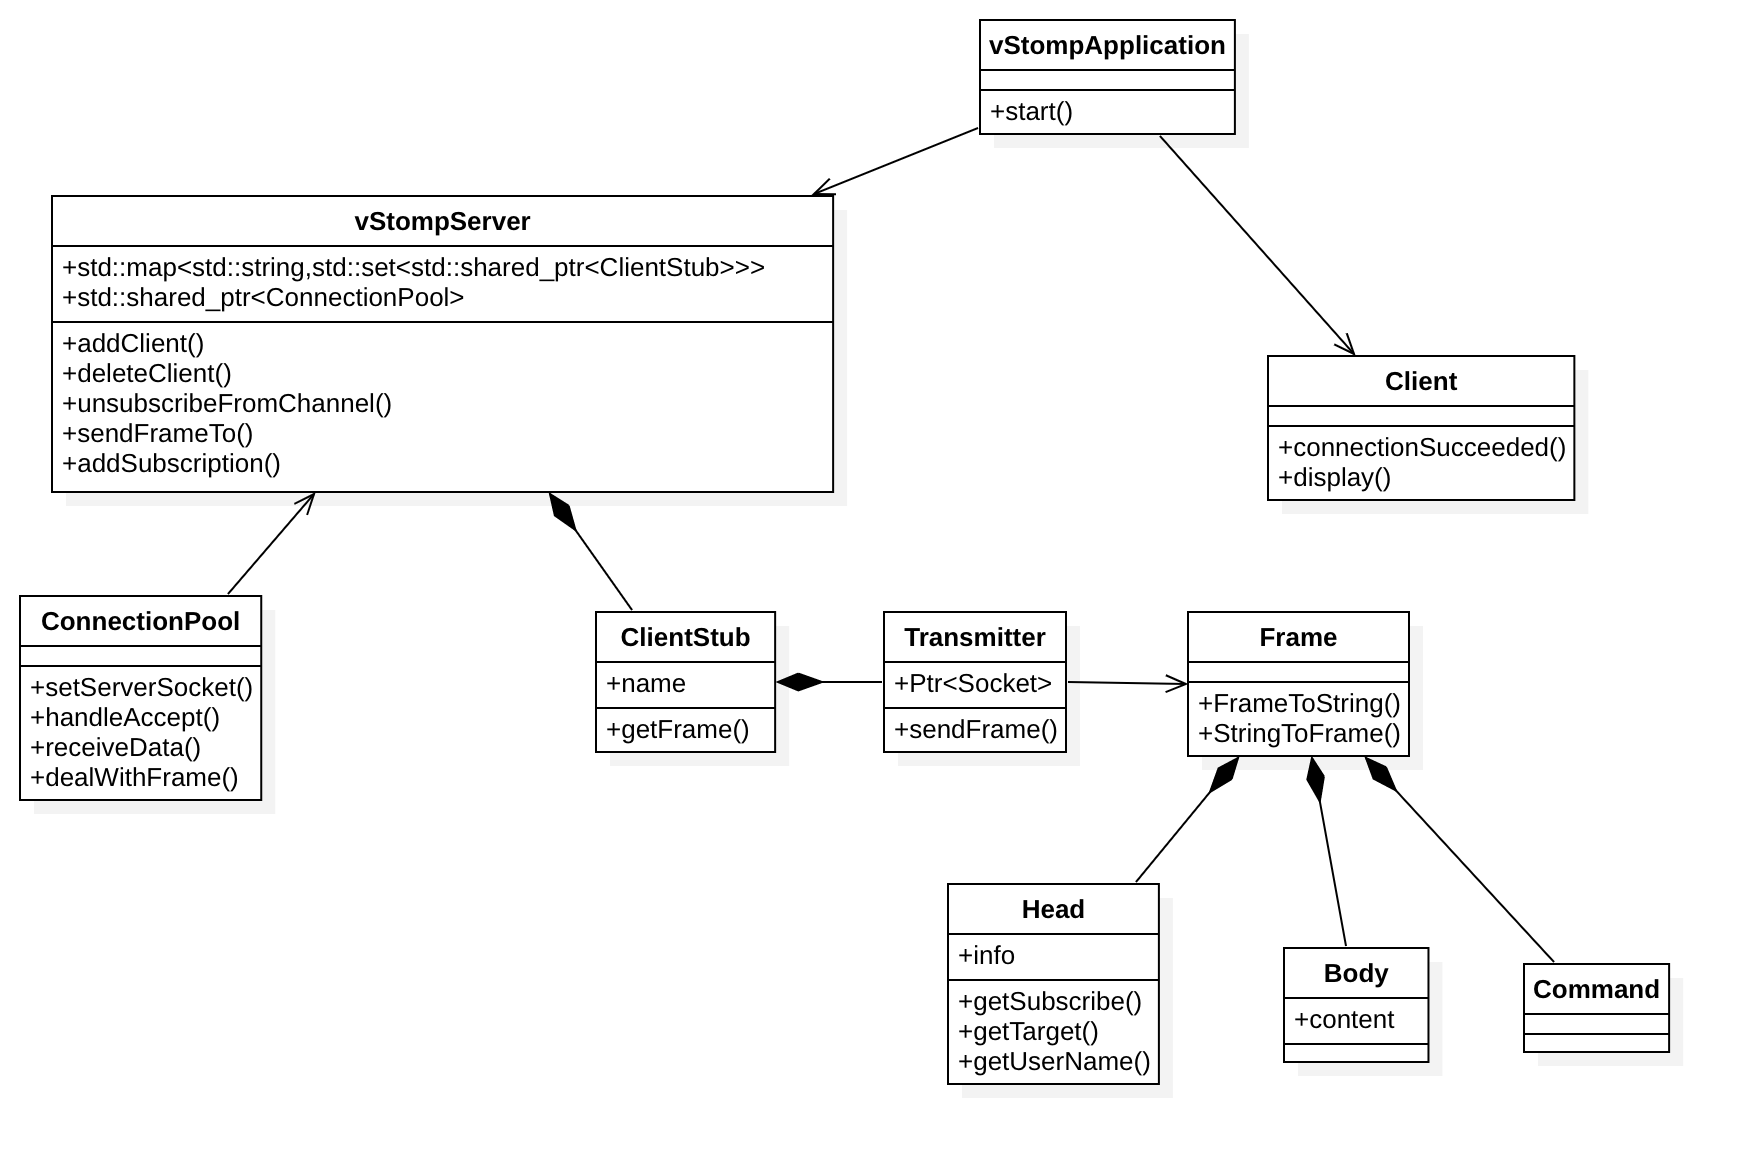
\includegraphics[width=0.86\linewidth]{img/Main}
		\caption{vStomp基本类型}
		\label{fig:main}
	\end{figure}
	在我们的系统开始运行之后,将会进行类似于下图的输出:\begin{figure}[H]
		\centering
		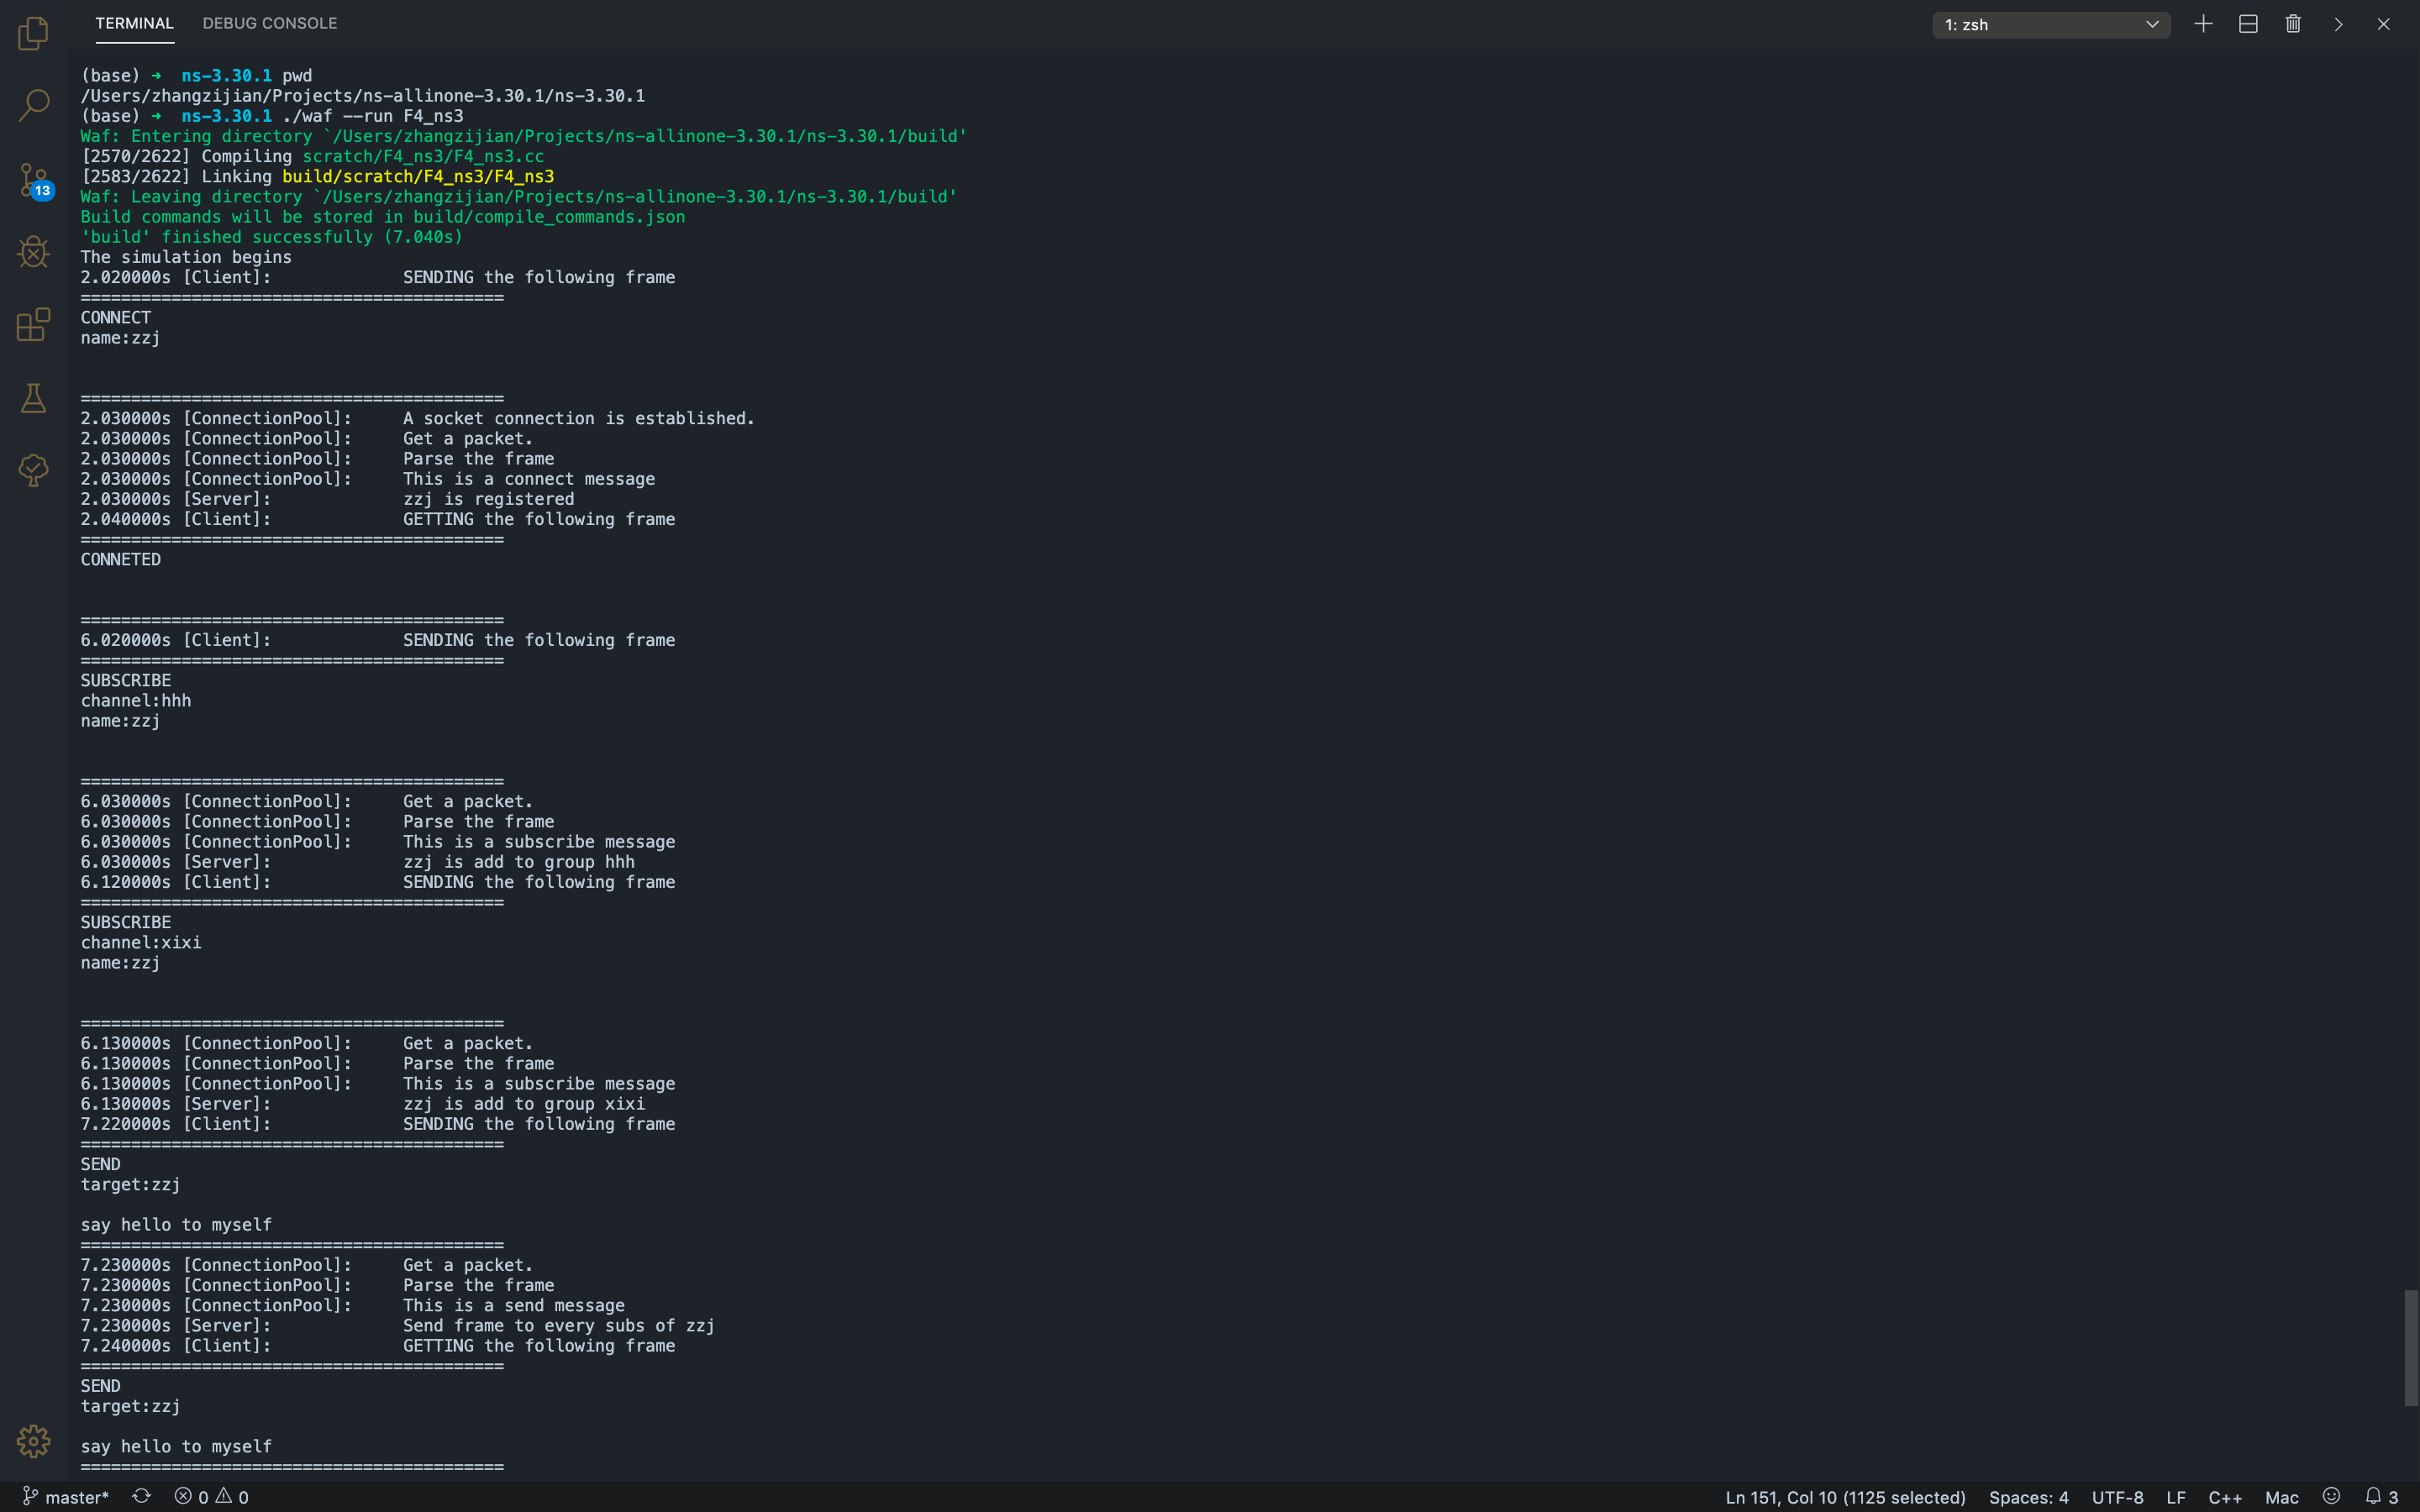
\includegraphics[width=0.86\linewidth]{img/programOutput}
		\caption{系统输出}
		\label{fig:programoutput}
	\end{figure}其中可以清晰看到我们发送的帧的格式与内容。这些内容都是真实发送的,使用的NS\_LOG\_INFO来进行的输出,具体处理可以到代码中查看。限于篇幅,不对每个类进行单独介绍,但是对于较为重要的设计我们将进行必要的描述。
	\section{Frame}
	Frame类就是我们的vStomp帧在内存中的具体表现,我们书写了它的序列化与反序列化函数,分别是FrameToString()与StringToFrame(),这两个函数的具体实现可以查看代码 frame.h。与之相关的类型定义如下所示:\begin{lstlisting}[language=c++]
enum Command{
 CONNECT,
 CONNECTED,
 SUBSCRIBE,
 SEND,
 DISCONNECT,
 UNSUBSCRIBE,
};

class Head{
 public:
   std::string getSubscribe();
   std::string getTarget();
   std::string getUserName();
 private: 
    std::map<std::string, std::string> info;
};

class Body{
 public:
   std::string content;
};
class Frame{
 public:
   Command command;
   Head head;
   Body body;
};
	\end{lstlisting}
	\section{ConnectionPool}
	为了适应ns-3中大量的回调机制,我们将服务器做了必要的切分来控制复杂性。有关用户的所有信息都是放置在vStompServer中的(具体表现为它内部存储的那个哈希表,记录这channel名称与该channel下的用户集合,而用户在我们的Server中表达被为ClientStub),而ConnectionPool则会负责具体应对用户的连接,它将会取出用户发送的信息,并根据用户的命令来调用vStompServer中的函数,从而完成相应的目标。我们可以在ConnectionPool最主要的函数中清晰看到上设计方式\begin{lstlisting}[language=c++]
void dealWithFrame(Frame frame,Ptr<Socket> socket){
 NS_LOG_INFO(std::to_string(Simulator::Now().GetSeconds()) +"s ["+ CLASSNAME +"]:     " + "Parse the frame");
 switch ((frame.command))
 {
  case CONNECT:{
	NS_LOG_INFO(std::to_string(Simulator::Now().GetSeconds()) +"s ["+ CLASSNAME +"]:     " + "This is a connect message");
	Transmitter transmiter(socket);
	std::shared_ptr<ClientStub> client(new ClientStub(transmiter,frame.head.getUserName()));
	server->addClient(client);
	Frame frame;
	frame.command = CONNECTED;
	client->getFrame(frame);
 }break;
 case SUBSCRIBE:{
	NS_LOG_INFO(std::to_string(Simulator::Now().GetSeconds()) +"s ["+ CLASSNAME +"]:     " + "This is a subscribe message");
	server->addSubscription(frame.head.getUserName(),frame.head.getSubscribe());
 }break;
 case SEND:{
	NS_LOG_INFO(std::to_string(Simulator::Now().GetSeconds()) +"s ["+ CLASSNAME +"]:     " + "This is a send message");
	server->sendFrameTo(frame.head.getTarget(), frame);
 }break;
 case DISCONNECT:{
	NS_LOG_INFO(std::to_string(Simulator::Now().GetSeconds()) +"s ["+ CLASSNAME +"]:     " + "This is a disconnect message");
	server->deleteClient(frame.head.getUserName());
 }break;
 case UNSUBSCRIBE:{
	NS_LOG_INFO(std::to_string(Simulator::Now().GetSeconds()) +"s ["+ CLASSNAME +"]:     " + "This is a unsubscribe message");
	server->unsubscribeFromChannel(frame.head.getUserName(), frame.head.getSubscribe());
 }break;
 default:
 break;
 }
}
	\end{lstlisting}
	下面再通过当服务器收到用户的SUBSCRIBE命令时的表现以及DISCONNECT命令时所做出的操作来进一步的展示我们的系统
	\begin{lstlisting}[language=c++]
void addSubscription(std::string userName, std::string channelName){
// the client automatically subscribe to a channel with the name of himself
  std::set<std::shared_ptr<ClientStub>> temptClient = clientPool[userName];
  std::shared_ptr<ClientStub> client = *(temptClient.begin());
  std::set<std::shared_ptr<ClientStub>> channelSubsribers = clientPool[channelName];
  channelSubsribers.insert(client);
  clientPool[channelName] = channelSubsribers;
  NS_LOG_INFO(std::to_string(Simulator::Now().GetSeconds()) +"s ["+ CLASSNAME +"]:             " + userName +" is add to group " + channelName);
}
void deleteClient(std::string clientName){
  for(auto iter = clientPool.begin();iter!=clientPool.end();){
   if(iter->first == clientName){
    clientPool.erase(iter ++ );
   }else{
    std::set<std::shared_ptr<ClientStub>> subscribers = iter->second;
    for(auto subsIter = subscribers.begin();subsIter!=subscribers.end();){
     if((*subsIter)->getName()==clientName){
      NS_LOG_INFO(std::to_string(Simulator::Now().GetSeconds()) +"s ["+ CLASSNAME +"]:             " + clientName + " unsubscribe " + iter->first);
      subscribers.erase(subsIter++);
      iter->second = subscribers;
      break;
     }else{
      subsIter ++;
     }
   }
  iter ++;
  }
 }
 NS_LOG_INFO(std::to_string(Simulator::Now().GetSeconds()) +"s ["+ CLASSNAME +"]:             " + clientName + " is leaving.");
}
	\end{lstlisting}
	\chapter{实验心得}
	首先感谢金老师在这2019-2020学年秋季学期计算机网络与计算机网络实验课程中的指导和帮助。
	
	这次自选实验标志着我们的计算机网络实验课程的结束,与前面所做的6次物理实验不同,最后这次实验我们使用的是虚拟的ns-3软件包来进行的。我们克服了一些困难,也获得了不少的收获。最主要的问题在于\begin{itemize}
		\item 语言的障碍。虽然我们在大一下学期有专门学习过一学期的C++语言,但是在课程结束之后就几乎没有再使用过,而C++本身又是如此复杂而令人困惑的。在完成ns-3自选实验的过程中,我们使用了不少特别的语言机制,其中最重要的就是回调函数的函数指针,我们确实感到陌生。在经过本次实验之后,我们有重新了解了有关的知识,增进了对C++的理解和掌握。
		\item 对如何实现一个协议的困惑。虽然现在想起来较为直观,无非就是对帧做序列化和反序列化,然后根据语义要求来进行必要的操作,但是在刚刚开始的时候我们确实对此感到迷茫。最终我们在Stomp的官网上找到了有关Stomp协议的开源实现,里面有一个非常简单的叫做Gozirra (\url{http://www.germane-software.com/software/Java/Gozirra/}),是一个Java的实现,我们对它进行了研究,并最终做出了我们的vStomp实现。
	\end{itemize}
\end{document}